\section{灵敏度分析与模型检验}

\subsection{灵敏度分析方法}

为评估模型关键参数对吨氨成本的影响程度，采用单因素扰动法进行灵敏度分析。以产量54吨/日为基准方案，依次对风电装机容量、光伏装机容量、购电电价、售电电价和储能投资成本五个参数进行$\pm$20\%--50\%的扰动，计算每个参数变化时吨氨成本的响应。灵敏度指标定义为参数变化$\pm$20\%时成本变化的百分比。

\subsection{灵敏度分析结果}

各参数的灵敏度分析结果如表\ref{tab:sensitivity}所示，龙卷风图如图\ref{fig:sensitivity}所示。

\begin{table}[H]
\centering
\caption{关键参数灵敏度分析结果}\label{tab:sensitivity}
\begin{tabular}{lccc}
\toprule
参数 & 扰动范围 & 成本变化范围(元/吨) & 灵敏度(\%) \\
\midrule
购电电价 & $\pm$30\% & 990.27 & 21.68 \\
光伏装机容量 & $\pm$20\% & 584.20 & 12.79 \\
风电装机容量 & $\pm$20\% & 236.44 & 5.18 \\
售电电价 & $\pm$30\% & 161.81 & 3.54 \\
储能投资成本 & $\pm$50\% & 1.22 & 0.03 \\
\bottomrule
\end{tabular}
\end{table}

\begin{figure}[H]
\centering
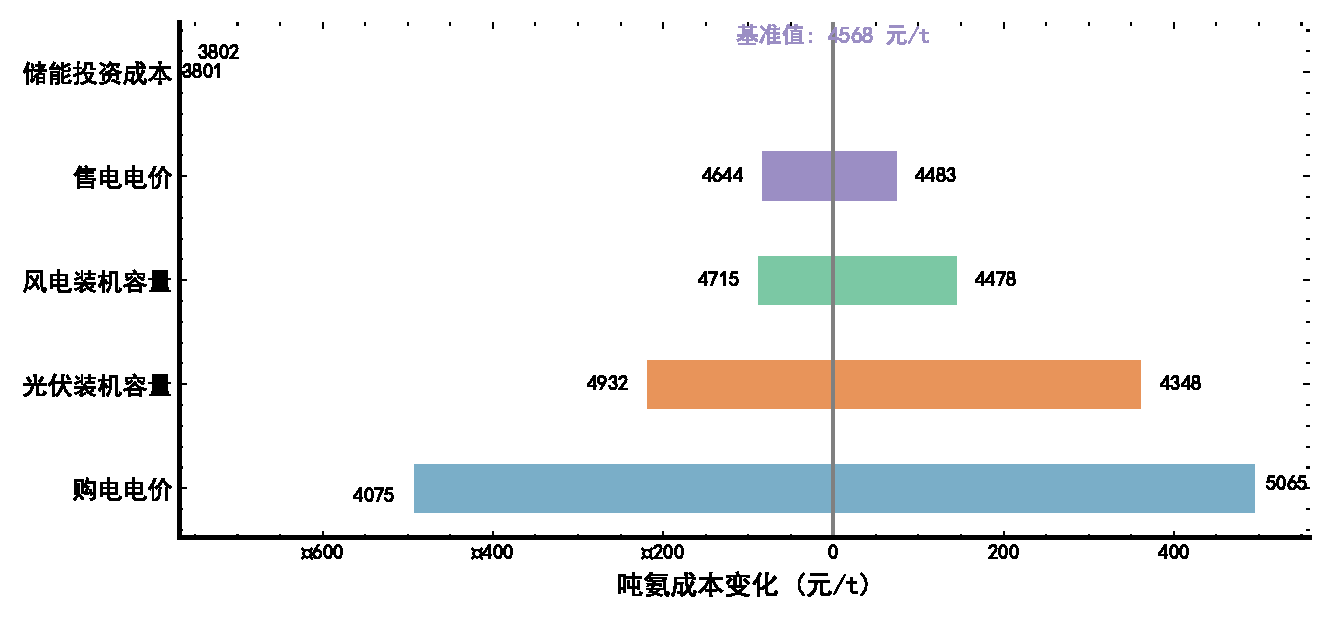
\includegraphics[width=0.85\textwidth]{../figures/fig_sensitivity.pdf}
\caption{关键参数敏感性分析龙卷风图}\label{fig:sensitivity}
\end{figure}

购电电价是影响吨氨成本最敏感的参数（灵敏度21.68\%），当购电电价在基准值的70\%至130\%范围内变化时，吨氨成本从4074.52元/吨变化到5064.79元/吨，变化幅度达990.27元/吨。这一结论符合物理直觉：购电成本在总成本中占比较高，且园区在夜间必须依赖电网购电维持生产。

光伏装机容量的灵敏度（12.79\%）显著高于风电装机容量（5.18\%），原因在于光伏的日发电量（358.4~MWh）大于风电（245.05~MWh），且光伏出力集中在白天生产高峰期，对自发自用比例的影响更为直接。售电电价的灵敏度较低（3.54\%），因为售电收入在总成本结构中占比有限。储能投资成本几乎不影响吨氨成本（灵敏度0.03\%），这是因为储能日折旧分摊到产氨量后数值极小。

\subsection{模型检验}

\subsubsection{能量守恒验证}

对所有问题的计算结果进行能量守恒检验。根据功率平衡方程，应满足$E_{\text{use}} + E_{\text{sell}} = E_{\text{RE}} + E_{\text{buy}}$。以问题一为例：$558.72 + 216.77 = 603.45 + 172.04$，即$775.49 = 775.49$，误差小于0.01~MWh，验证通过。

\subsubsection{约束满足验证}

检验所有优化结果是否满足问题约束：（1）功率非负：所有$P_{\text{buy}}(t) \geq 0$、$P_{\text{sell}}(t) \geq 0$均满足；（2）产量约束：各产量方案的实际产氨量与目标值完全一致；（3）出力系数范围：问题三中所有$\alpha(t) \in [0, 1]$，不存在越界情况；（4）SOC范围：问题四中所有时段$0.1 C_{\text{bat}} \leq E(t) \leq 0.9 C_{\text{bat}}$均满足。

\subsubsection{资源单调性验证}

验证"更多资源$\to$更优结果"的单调性：（1）问题三的成本$\leq$问题二的成本（连续可行域包含离散可行域），所有产量均验证通过；（2）有储能的产量$\geq$无储能的产量（储能增加了调度灵活性），验证通过；（3）联网产量$\geq$离网产量（电网提供了额外的电力来源），验证通过。
